% Relatório em LaTeX para o trabalho de PPC Autor: Daniel Martins Cabrita de
% Sousa Data: Outubro 2025
\documentclass[a4paper,openright,twoside,11pt]{report}

% Packages utilizadas e respetivos parâmetros.
\usepackage[utf8]{inputenc}
\usepackage[english]{babel}
\usepackage{amsmath}  
\usepackage{graphicx}
\usepackage{url}
\usepackage[Algoritmo]{algorithm}
\usepackage{algorithmicx}
\usepackage{algpseudocode}
\usepackage{acronym}
\usepackage{float}

\usepackage{listings}
\usepackage{xcolor}
\usepackage{enumitem}
\usepackage{booktabs}
\usepackage[hidelinks]{hyperref}


\setlist[itemize]{itemsep=0pt, topsep=3pt}

% Índice
\usepackage{makeidx}
\makeindex

% Definições das dimensões das páginas
\setlength{\textheight}{24.00cm}
\setlength{\textwidth}{15.50cm}
\setlength{\topmargin}{0.35cm}
\setlength{\headheight}{0cm}
\setlength{\headsep}{0cm}
\setlength{\oddsidemargin}{0.25cm}
\setlength{\evensidemargin}{0.25cm}

%\renewcommand{\baselinestretch}{1}

% Página inicial (capa)
\title{
   \vspace{-50mm}
   \begin{minipage}[l]{\textwidth}
      \hspace{-20mm}\resizebox{75mm}{!}{
\includegraphics{images/fcul.png}}\\
   \end{minipage}\\[20mm]
   \textbf{Kloud Motors} 
   \\
   Online Car Dealer
}

% Nome dos autores (um por linha)
\author{
\begin{tabular}{ll}
             & Daniel Martins Cabrita de Sousa: 66128  \\
             & Daniel Alexandre Marto Queijo de Carvalho: 66208  \\
             & Daniel Ribeiro Nunes: 66462 \\
             & Francisco Lopes da Encarnação: 66131  \\
\end{tabular}}

\date{
\begin{tabular}{ll}
  {Professor:} & Mário Calha \end{tabular}\\[10mm]
Assignment report for Cloud Computing \\
MSc in Computer Engineering \\[5mm]
GitHub repository: \url{https://github.com/cheestree/comp-nuvem-2026} \\[45mm] June 2026}


\begin{document}
\pagenumbering{roman}
\thispagestyle{empty}
\maketitle

\baselineskip 18pt 
\newpage
\thispagestyle{empty}
% Fim da contracapa

\cleardoublepage
\tableofcontents \cleardoublepage

% Reiniciar a numeração de páginas
\setcounter{page}{1}
\pagenumbering{arabic}


\chapter{Introduction} \label{chap:introduction}

Kloud Motors is a cloud computing project that implements an online car dealer platform over a large vehicle-listing dataset. The goal of the project is not only to expose marketplace data through an HTTP API, but also to design and operate the platform as a \textbf{cloud-native system} composed of independent services, databases, deployment scripts, and infrastructure configuration. The application therefore combines a realistic business domain, \textit{used and new car sales}, with the technical concerns expected from distributed cloud applications: service decomposition, database isolation, public API design, real-time communication, observability, containerization, Kubernetes deployment, and automated infrastructure support.

\section{Motivation}

Vehicle marketplaces are naturally data-intensive systems. A user looking for a car rarely needs only a static catalogue entry: they compare similar listings, filter by price or mileage, inspect the seller, check whether prices vary by region, save interesting options, and sometimes interact directly with the seller before deciding. Sellers, on the other hand, need ways to expose listings, manage their lifecycle, and potentially use alternative sale formats such as auctions. These requirements make the domain a suitable case study for a cloud platform because it contains both read-heavy analytical workloads and interactive user workflows.

The project was motivated by this combination of marketplace functionality and cloud engineering challenges. A monolithic implementation would be simpler, but it would hide many of the concerns that become important when an application must \textbf{scale, evolve, and tolerate failures}. Kloud Motors was therefore designed around a \textbf{REST and WebSocket gateway} backed by internal gRPC microservices. This makes it possible to separate responsibilities such as listing search, market analysis, user accounts and authentication, seller profiles, chat, and auctions while preserving a single public entry point for clients.

\section{Dataset Characterization}

The platform is based on the \textit{Large Car Dataset} published on Kaggle, a dataset containing used and new car marketplace listings. The dataset has an approximate size of \texttt{5.3 GB} and was published in 2020, with updates in 2021. Its domain fits the project because each record represents the kind of information expected in a car marketplace: vehicle make and model, year, price, mileage, fuel type, location, seller-related information, technical specifications, and listing state.

In the project workflow, the dataset is prepared locally through the scripts in \texttt{scripts/local/} and then loaded into the PostgreSQL databases used by the services. During preparation, the original columns are normalised into fields such as \texttt{VIN}, price, mileage, new/sold state, brand, model, model year, body class, fuel type, transmission, drive type, engine data, colour, seller identifier, and generated location fields. The listing database acts as the \textbf{main source of truth} for catalogue browsing, search, listing details, comparison, market price calculations, and geographical market insights. This structure allows the same base data to support different user facing operations: simple retrieval for listing pages, filtered retrieval for search, aggregation for market analysis, and grouping by city, state, country, or district fields for regional insights.

\section{Business Capabilities}

Kloud Motors exposes a set of business capabilities that together model an online car marketplace. The \textbf{catalogue} capability allows users to retrieve detailed vehicle listings and compare multiple cars side by side. The \textbf{search} capability supports filters such as make, model, year, price range, mileage, fuel type, pagination, and sold-state inclusion, enabling users to narrow a large dataset into relevant results.

The platform also includes analytical capabilities. \textbf{Market price analysis} computes average price information for a selected brand and model, optionally restricted by year ranges. \textbf{Geographical market insights} compare prices and availability across supported location fields, giving users a view of how the same vehicle behaves in different markets. These capabilities turn the dataset from a simple list of cars into decision-support information for buyers and sellers.

Beyond catalogue and analysis features, the application supports marketplace interaction. Seller profiling exposes information about the actor behind a listing. User registration, login, and token refresh are handled by the user service through Firebase authentication, while the gateway validates Firebase ID tokens before forwarding protected requests. Registered users can manage favourite listings. Buyer-seller communication is implemented through chat sessions associated with listings, including WebSocket-based real-time messaging. Chat indexing is stored in PostgreSQL, message persistence is backed by Firestore, and Google Pub/Sub can distribute real-time events across replicas. The auction module adds another transactional workflow by allowing authenticated sellers to create auctions and authenticated buyers to place bids while clients receive live auction updates, also with Pub/Sub support for distributed WebSocket updates.

\section{Use Cases}

The main use cases follow directly from these capabilities. A visitor can search the catalogue using filters and inspect detailed listings before comparing selected cars. A buyer interested in fair pricing can request average market prices for a specific brand and model, while another user can compare prices by location to understand regional differences. When a listing is promising, the visitor can inspect the seller profile, register or log in through the \texttt{/api/user} routes, save the listing as a favourite through the protected \texttt{/api/users/me/favorites} routes, and open a chat with the seller.

The platform also supports seller-oriented and real-time scenarios. Authenticated users can create, update, or delete listings through the gateway. Sellers can create auctions for specific listings, buyers can place bids, and authenticated clients can receive auction updates over WebSockets. These use cases exercise both the data-oriented and interactive parts of the system, making Kloud Motors a representative cloud application rather than a purely static API over a dataset.

The remainder of this report presents the API contract, functional and non-functional requirements, service architecture, implementation details, deployment model, pipeline, validation strategy, future improvements, and cost analysis of the Kloud Motors platform.


\chapter{API specification} \label{cap:api}

The Kloud Motors API follows a RESTful architecture. The endpoints have been categorized by their primary domain, such as User Management, Chat, Auctions, and Listings. Each table provides the HTTP method, the endpoint path, and a brief description of its functionality. The full OpenAPI specification file is provided as a separate attachment in .yaml format.

\subsection{Users}
\begin{table}[htpb]
\centering
\begin{tabular}{p{1.8cm} p{6.5cm} p{6.5cm}}
\toprule
\textbf{Method} & \textbf{Endpoint} & \textbf{Description} \\
\midrule
POST & /api/user/login & Authenticate a user with email and password \\
POST & /api/user/register & Register a user with email and password \\
POST & /api/user/refresh & Refresh a Firebase ID token \\
GET* & /api/users/me/favorites & Get the authenticated user's favorite listing IDs \\
POST* & /api/users/me/favorites/\{listing\_id\} & Add a listing to favorites \\
DELETE* & /api/users/me/favorites/\{listing\_id\} & Remove a listing from favorites \\
POST & /api/users/preview & Get user previews \\
\bottomrule
\multicolumn{3}{l}{\small \textit{* Requires Bearer Token authentication}}
\end{tabular}
\caption{User Management Endpoints}
\label{tab:api_users}
\end{table}

\subsection{Chat}
\begin{table}[htpb]
\centering
\begin{tabular}{p{1.8cm} p{6.5cm} p{6.5cm}}
\toprule
\textbf{Method} & \textbf{Endpoint} & \textbf{Description} \\
\midrule
GET* & /api/chat & Get user chats \\
POST* & /api/chat/open & Open or create a buyer-seller chat session \\
GET* & /api/chat/\{chat\_id\} & Get chat history \\
GET* & /api/chat/ws/\{chat\_id\} & Chat WebSocket proxy \\
\bottomrule
\multicolumn{3}{l}{\small \textit{* Requires Bearer Token authentication}}
\end{tabular}
\caption{Buyer-Seller Communication Endpoints}
\label{tab:api_chat}
\end{table}

\subsection{Market Insights \& Price Analysis}
\begin{table}[htpb]
\centering
\begin{tabular}{p{1.8cm} p{6.5cm} p{6.5cm}}
\toprule
\textbf{Method} & \textbf{Endpoint} & \textbf{Description} \\
\midrule
GET & /api/market/insights/aggregates & Get aggregated market insights \\
GET & /api/market/price-comparison & Compare prices across locations \\
GET & /api/listings/stats/by-location & Get listing price statistics by location \\
GET & /api/market/average-price & Get average market price \\
\bottomrule
\end{tabular}
\caption{Geographical Market Insights and Pricing Endpoints}
\label{tab:api_market}
\end{table}

\subsection{Auctions}
\begin{table}[htpb]
\centering
\begin{tabular}{p{1.8cm} p{6.5cm} p{6.5cm}}
\toprule
\textbf{Method} & \textbf{Endpoint} & \textbf{Description} \\
\midrule
GET & /api/auctions & List auctions \\
POST* & /api/auctions & Create an auction \\
GET & /api/auctions/\{auction\_id\} & Get auction details \\
DELETE* & /api/auctions/\{auction\_id\} & Delete an auction \\
POST* & /api/auctions/\{auction\_id\}/bid & Place a bid \\
GET & /api/auctions/\{auction\_id\}/bids & Get auction bids \\
GET* & /api/auctions/ws/\{auction\_id\} & Auction WebSocket proxy \\
\bottomrule
\multicolumn{3}{l}{\small \textit{* Requires Bearer Token authentication}}
\end{tabular}
\caption{Auction Module Endpoints}
\label{tab:api_auctions}
\end{table}

\subsection{Sellers}
\begin{table}[htpb]
\centering
\begin{tabular}{p{1.8cm} p{6.5cm} p{6.5cm}}
\toprule
\textbf{Method} & \textbf{Endpoint} & \textbf{Description} \\
\midrule
GET & /api/sellers/\{seller\_id\} & Get seller profile \\
POST & /api/sellers/preview & Get seller previews \\
\bottomrule
\end{tabular}
\caption{Seller Management Endpoints}
\label{tab:api_sellers}
\end{table}

\subsection{Listings}
\begin{table}[htpb]
\centering
\begin{tabular}{p{1.8cm} p{6.5cm} p{6.5cm}}
\toprule
\textbf{Method} & \textbf{Endpoint} & \textbf{Description} \\
\midrule
GET & /api/listings & Get listings \\
POST* & /api/listings & Create a listing \\
GET & /api/listings/search & Search listings \\
GET & /api/listings/compare & Compare listings \\
GET & /api/listings/\{id\} & Get listing details \\
PUT* & /api/listings/\{id\} & Update a listing \\
DELETE* & /api/listings/\{id\} & Delete a listing \\
\bottomrule
\multicolumn{3}{l}{\small \textit{* Requires Bearer Token authentication}}
\end{tabular}
\caption{Filtered Search and Listing Endpoints}
\label{tab:api_listings}
\end{table}
\chapter{Functional and non-functional requirements} \label{cap:requirements}
\chapter{Architecture} \label{cap:architecture}

Kloud Motors follows a microservices architecture implemented in Go. The public surface of the application is a REST and WebSocket gateway, while the internal services communicate through gRPC. The same service decomposition is used for local execution with Docker Compose and for cloud execution on Kubernetes.

\section{Application Architecture}

At application level, the platform is organised around a single gateway and a set of domain services. Clients do not call the internal services directly. Instead, all HTTP routes under \texttt{/api} and all public WebSocket routes are received by the gateway. The gateway validates requests, verifies Firebase ID tokens for protected operations, maps HTTP requests into gRPC calls, and proxies WebSocket connections for chat and auctions.

The main application services are:

\begin{itemize}
    \item \textbf{Gateway service}: exposes the REST API, WebSocket entry points, health endpoint, metrics endpoint, Firebase token validation, and gRPC clients for downstream services.
    \item \textbf{Listing service}: owns listing details, listing summaries, comparison, listing creation, update, deletion, ownership checks, and sold state checks.
    \item \textbf{Search service}: provides paginated listing search over the listing database and caches repeated search results in Redis.
    \item \textbf{Market price service}: computes average, minimum, and maximum market prices for a selected brand and model.
    \item \textbf{Geographical market insights service}: provides aggregate, price-comparison, and by-location statistics grouped by district, city, or country.
    \item \textbf{User service}: handles Firebase-backed registration, login, token refresh, internal user resolution, user previews, and favourite listings.
    \item \textbf{Seller service}: provides seller profiles and seller previews.
    \item \textbf{Chat service}: manages chat creation, chat listing, chat history, and live buyer-seller messaging.
    \item \textbf{Auction service}: manages auction listing, creation, detail retrieval, deletion, bidding, bid retrieval, and live auction updates.
\end{itemize}

The application data is separated by concern. The listing database is shared by read heavy marketplace services because listing, search, market price, and geographical insights all operate over the same vehicle data. User, seller, chat, and auction state are stored in separate PostgreSQL databases. Chat also uses Firestore for message persistence when configured. Redis is used as a cache aside layer for listing detail, listing summary, and search query results. Google Pub/Sub is used by chat and auction services to distribute real-time WebSocket events across replicas.

\section{Technical Architecture}

The services are containerised and deployed to Kubernetes under the \texttt{vehicles-prod} namespace. The top-level Kustomize configuration includes the namespace, shared service account, Cloud SQL configuration, gateway, all domain services, Redis, backup resources, and ingress. The ingress accepts traffic for \texttt{kloud-motors.com} and routes \texttt{/api/}, \texttt{/api/chat/ws/}, and \texttt{/api
/auctions/ws/} to the gateway service.

Inside Kubernetes, service discovery is performed through Kubernetes service names. The gateway receives downstream addresses from its ConfigMap, including \texttt{listing-service:50054}, \texttt{search-service:50056}, \texttt{user-service:50058}, \texttt{seller-service:50057}, \texttt{chat-service:50052}, \texttt{marketprice-service:50055}, \texttt{geographic-market-insights-service:50053}, and \texttt{auction-
service:50051}. WebSocket upstreams are configured separately as \texttt{ws://chat-service:8080} and \texttt{ws://auction-service:8081}. Several cross-cutting technical mechanisms are implemented in the codebase:

\begin{itemize}
    \item \textbf{Authentication}: the user service calls Firebase Identity Toolkit and Secure Token APIs for registration, login, and refresh. The gateway verifies Firebase ID tokens and resolves them to internal user IDs.
    \item \textbf{Resilience}: the gateway wraps downstream gRPC clients with circuit breakers. Chat and auction also wrap selected listing and seller service calls with circuit breakers.
    \item \textbf{Observability}: the gateway exposes \texttt{/metrics} for Prometheus and \texttt{/api/health} for health checks. HTTP and gRPC boundaries are instrumented with OpenTelemetry in the gateway and main services.
    \item \textbf{Scalability}: services have Kubernetes deployment and service manifests, and scalable services define HorizontalPodAutoscaler resources. Redis reduces database load for repeated read paths, while Pub/Sub enables horizontally scaled WebSocket delivery.
    \item \textbf{Backup}: a Kubernetes CronJob exports configured Cloud SQL databases to Google Cloud Storage.
    \item \textbf{Infrastructure as code}: Terraform defines core GCP resources, including Cloud SQL, a backup bucket, Artifact Registry, Pub/Sub topics, service accounts, VPC networking, and GKE resources.
    \item \textbf{Automation}: GitHub Actions runs Go unit tests, Docker Compose based integration tests, and Terraform validation/deployment workflows.
\end{itemize}

\section{Architecture Diagram}

Figure~\ref{fig:architecture} summarises the connection between the client, gateway, services, data stores, messaging infrastructure, observability stack, deployment automation, and cloud infrastructure.

\begin{figure}[p]
    \centering
    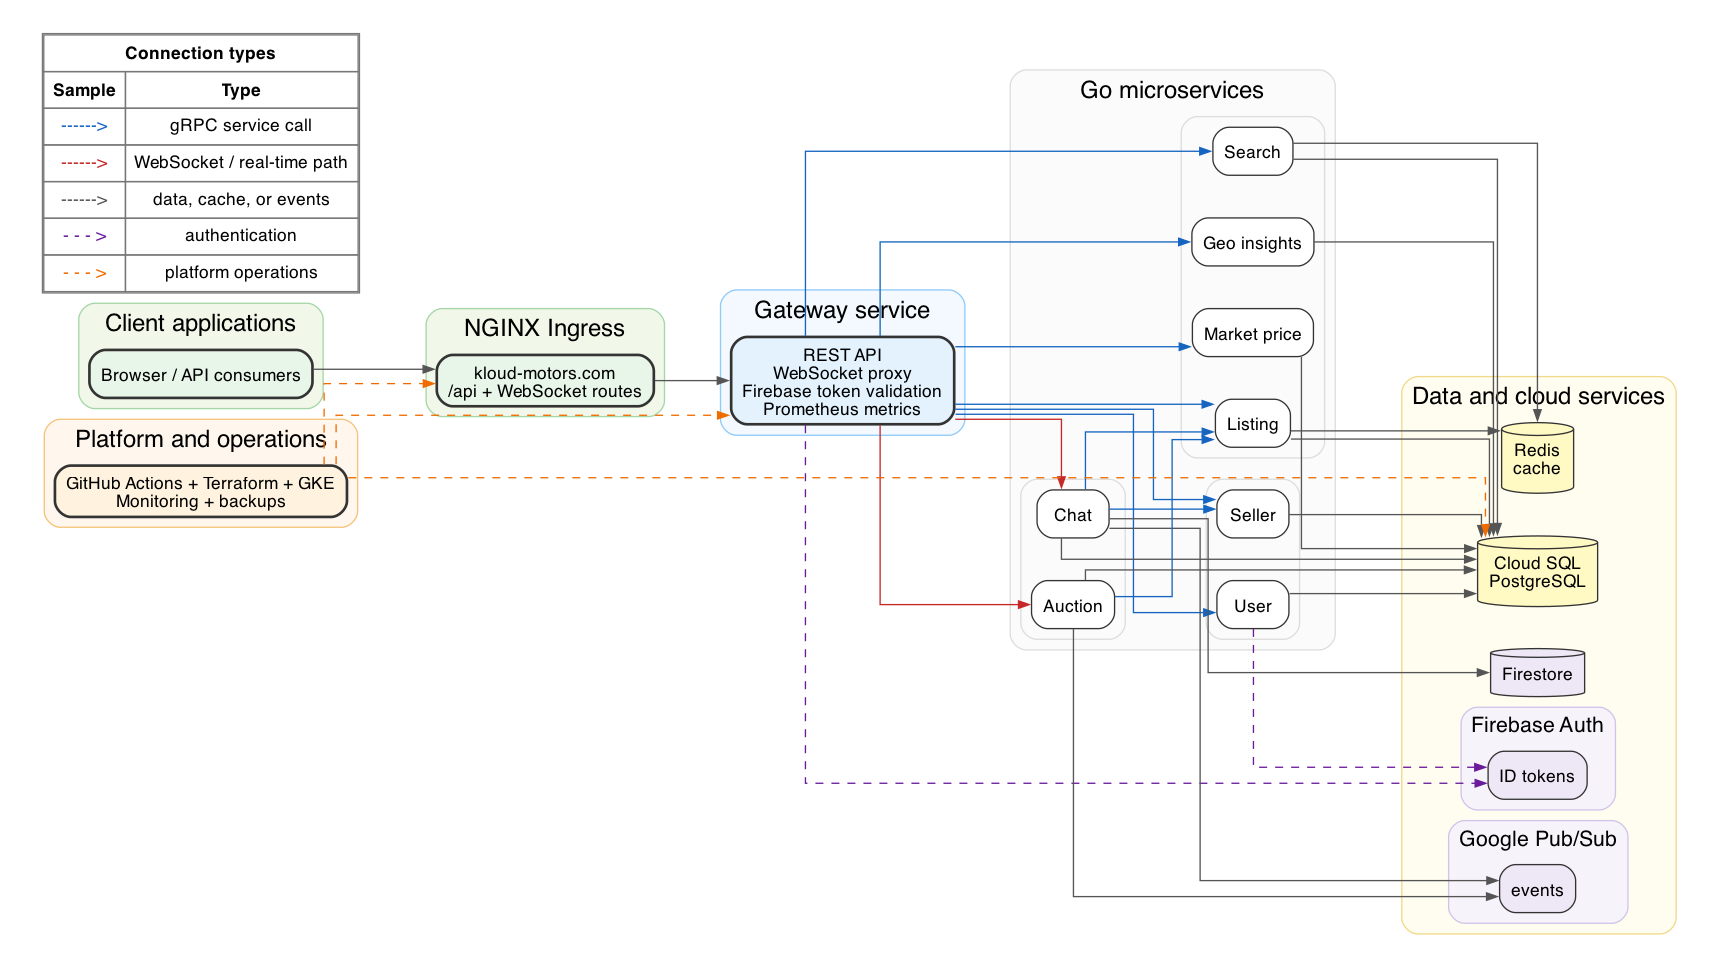
\includegraphics[angle=90,width=\textwidth,height=0.78\textheight,keepaspectratio]{architecture/images/architecture.png}
    \caption{Kloud Motors application and technical architecture}
    \label{fig:architecture}
\end{figure}

\chapter{Implementation} \label{cap:implementation}
\chapter{Deployment scripts and tuning} \label{cap:deployment}

The deployment process was automated around two complementary concerns: creating the cloud infrastructure in a repeatable way and updating the Kubernetes workloads with minimal manual intervention. The repository therefore separates infrastructure provisioning, image publication, application deployment, monitoring, and backup operations into scripts under the \texttt{scripts/cloud} directory and declarative manifests under \texttt{deploy/k8s}.

\section{Infrastructure bootstrap}

The cloud layer is managed with Terraform. Before it is executed, the Terraform initialization script creates, when necessary, a Google Cloud Storage bucket for the remote Terraform state and enables object versioning on it. The bucket name is derived from the active Google Cloud project, which keeps the Terraform backend consistent between machines.

The Terraform configuration provisions the main managed services used by the system: a PostgreSQL Cloud SQL instance, the individual microservice databases, an Artifact Registry Docker repository, Pub/Sub topics, a backup bucket, a VPC and subnet, and the GKE cluster. The cluster uses a custom node pool with \texttt{e2-standard-2} nodes and Workload Identity enabled, so microservice pods can access Google Cloud resources through a Kubernetes service account. This is also used by the backup CronJob and the Cloud SQL proxy sidecars.

\section{Image build and publication}

Container images are built and pushed by the \texttt{build\_and\_push.sh} script. The script iterates over all runtime services, including the gateway and other services like Redis. Each service image is built with Docker for the target platform (which defaults to \texttt{linux/amd64} that is the system Cloud Run containers must use), tagged with the Artifact Registry path, and pushed to the \texttt{vehicles} repository.

\section{Kubernetes deployment}

The workloads and other configurations are set as Kubernetes manifests and composed with Kustomize. The root \texttt{deploy/k8s/kustomization.yaml} applies the shared namespace, service account, Cloud SQL configuration, all microservice deployments and services, Redis, the backup CronJob and the ingress rule. To aid the Kubernetes deployment, a helper script was developed (\texttt{scripts/cloud/k8s.sh}) that wraps common operational actions:

\begin{itemize}
    \item \texttt{up}: Applies the Kubernetes manifests;
    \item \texttt{down}: Deletes the Kubernetes manifests;
    \item \texttt{status}: Shows the current pod and service status;
    \item \texttt{restart}: Restart all deployments (rollout restart).
\end{itemize}

The script detects the namespace from the manifest, selects the kubeconfig from CI or from the local project file, checks cluster connectivity, applies the manifests and optionally waits for rollouts to complete.

After applying manifests, the script restarts deployments so that pods pull the latest image tag from the Artifact Registry. Ingress can be managed through the same deployment flow. The ingress routes all \texttt{/api/} traffic to the gateway service, with explicit WebSocket paths for chat and auctions and longer proxy read/send timeouts to support persistent connections.

\section{Operational tuning}

Much of the performance tuning was done at the Kubernetes workload level. Each service defines CPU and memory requests and limits so the scheduler can place pods reliably on the small GKE node pool and so individual services cannot consume all cluster resources during stress tests. Lighter services like \texttt{user} use smaller requests, while listing or search reserve more CPU and memory because they perform heavier database queries or aggregation work. Services that connect to Cloud SQL include a Cloud SQL proxy sidecar with its own resource budget, preventing the proxy from competing invisibly with the application container. These values were tweaked after CloudyDay to better strengthen the infrastructure.

Readiness and liveness probes were added to the HTTP and gRPC-facing deployments. Readiness probes prevent Kubernetes services from sending traffic to pods before they have completed startup and dependency initialization. Liveness probes allow Kubernetes to restart pods that become unhealthy.

Horizontal Pod Autoscalers are configured for the stateless application services. Most services scale from one replica up to eight replicas using CPU and memory utilization targets of roughly 70\% and 80\%, respectively. The chat service uses slightly lower targets and a maximum of ten replicas because WebSocket traffic can keep pods busy even when request counts are not high. For services such as listing, search, seller, user, etc., the HPA behavior allows fast scale-up while applying a 180 second stabilization window when scaling-down (to avoid oscillation during short traffic spikes while still allowing the cluster to reduce cost after load decreases).

\section{Backup and monitoring support}

Database and dataset backup operations are also scripted. The manual \texttt{backup\_data.sh} script exports the Cloud SQL databases to Google Cloud Storage and uploads prepared dataset artifacts. There is also, in the cluster, a Kubernetes CronJob that runs daily at 02:00 UTC and exports the configured Cloud SQL databases to the backup bucket. The backup bucket has object versioning enabled and a lifecycle rule that moves older objects to Coldline storage after 30 days, reducing storage cost while keeping recovery points available.

Monitoring is deployed separately with the monitoring Kubernetes helper and use the manifests under \texttt{deploy/k8s/monitoring}. This includes Prometheus, Grafana, kube-state-metrics, services, RBAC rules, etc. Keeping monitoring in its own namespace and script allows restart, remove or inspect observability components without touching the application workloads. During tuning, the Prometheus and Grafana views were used to compare pod resource usage with the configured requests, limits and HPA thresholds after smoke and stress tests.
\chapter{CI/CD pipeline} \label{cap:pipeline}
\chapter{Group 16 Evaluation} \label{cap:tests}
\chapter{CloudyDay improvements} \label{cap:improvements}
\chapter{Cost analysis} \label{cap:costs}

\chapter{Conclusion} \label{cap:conclusion}

Kloud Motors achieved the main goal of the project: building a \textbf{cloud-native online car dealer platform} around a realistic vehicle dataset. The final system is not only an API over static data, but a distributed application composed of a public gateway, internal gRPC services, PostgreSQL databases, Redis caching, Firebase authentication, WebSocket-based real-time features, Pub/Sub event distribution, Kubernetes deployment manifests, Terraform infrastructure, monitoring, backups, and CI/CD automation.

The \textbf{microservices architecture} proved useful for separating the main business domains of the platform. Listing, search, market price, geographical insights, users, sellers, chat, and auctions can evolve independently while still being exposed through one public REST and WebSocket gateway. This structure also made it possible to introduce cross-cutting concerns in a controlled way: the gateway centralises public authentication and HTTP error mapping, services keep their internal gRPC contracts, Redis reduces repeated read pressure, and circuit breakers and timeouts help the system behave better when dependencies are slow or unavailable.

The deployment work was an important part of the project. The application can run locally with Docker Compose, but it is also prepared for cloud execution on GKE through Kubernetes manifests and Kustomize. Terraform defines the supporting Google Cloud resources, including Cloud SQL, Artifact Registry, Pub/Sub, Cloud Storage, service accounts, networking, and the GKE cluster. The CI/CD workflows connect these pieces by running Go tests, executing Docker Compose integration tests, applying Terraform changes, building and pushing service images, and rolling the workloads out to GKE.

The Cloudy Day and stress-test phase exposed several practical issues that are common in distributed systems. These tests motivated improvements in gateway validation, gRPC timeouts, circuit breakers, database indexes, resource requests and limits, HPA configuration, and operational documentation. As a result, the final version is more robust than the initial implementation and better aligned with the non-functional requirements of scalability, resilience, observability, and maintainability.

There are still limitations. The GKE node pool and Cloud SQL instance are intentionally small to keep the assignment cost under control, so the current deployment should be seen as a \textit{realistic prototype} rather than a production-sized system. The HPA configuration prepares services for horizontal scaling, but a production deployment would also require node autoscaling, stronger database capacity planning, stricter secret management, TLS configuration, image tag immutability, and more complete end-to-end tests for authenticated and real-time workflows.

Overall, the project demonstrates the \textbf{full lifecycle of a cloud application}: data preparation, API design, service implementation, containerisation, cloud infrastructure provisioning, Kubernetes deployment, automated validation, monitoring, backup, and cost-aware operation. The result is a working platform that satisfies the main functional requirements while also exercising the operational practices expected from a modern cloud computing system.



% \bibliographystyle{unsrt} \bibliography{referencias}
% \addcontentsline{toc}{chapter}{References}

% Apêndices (opcional)
% \appendix
% \include{appendix}

\end{document} 
